\documentclass[a4paper,oneside]{report}
%uncomment to see the references
%\usepackage{showkeys}

% \usepackage{bbm}
\usepackage[T2A]{fontenc}
\usepackage[utf8]{inputenc}

%\usepackage{expdlist}
\usepackage[pdftex]{graphicx}
\graphicspath{{pic/}}
\usepackage{amsmath, amssymb, amsthm}
\usepackage{amsfonts, amsxtra}

\usepackage{sty/dbl12}
\usepackage{epsfig}
\usepackage{verbatim}

\usepackage{sty/rac}
\usepackage{placeins}
\usepackage[english,russian]{babel}

% This handles the translation of unicode to latex:

\usepackage[section]{algorithm}
\usepackage{algorithmic}

\usepackage[backend=biber,bibencoding=utf8,sorting=none,sortcites=true,bibstyle=sty/gost71,maxnames=99,citestyle=numeric-comp,babel=other]{biblatex}

\defbibenvironment{bibliography}
  {\list
     {\printfield[labelnumberwidth]{labelnumber}.}
     {\setlength{\labelwidth}{2\labelnumberwidth}%
      \setlength{\leftmargin}{\labelwidth}%
      \setlength{\labelsep}{\biblabelsep}%
      \addtolength{\leftmargin}{\labelsep}%
      \setlength{\itemsep}{\bibitemsep}%
      \setlength{\parsep}{\bibparsep}}%
      \renewcommand*{\makelabel}[1]{\hss##1}}
  {\endlist}
  {\item}

\usepackage{csquotes}
%\usepackage[nottoc,notbib]{tocbibind}
% \usepackage{listings}

%%% FOR llbrace and rrbrace
\usepackage{accsupp} % for ensuring the right Unicode codepoint upon pasting
\newcommand*{\llbrace}{%
  \BeginAccSupp{method=hex,unicode,ActualText=2983}%
    \textnormal{\usefont{OMS}{lmr}{m}{n}\char102}%
    \mathchoice{\mkern-4.05mu}{\mkern-4.05mu}{\mkern-4.3mu}{\mkern-4.8mu}%
    \textnormal{\usefont{OMS}{lmr}{m}{n}\char106}%
  \EndAccSupp{}%
}
\newcommand*{\rrbrace}{%
  \BeginAccSupp{method=hex,unicode,ActualText=2984}%
    \textnormal{\usefont{OMS}{lmr}{m}{n}\char106}%
    \mathchoice{\mkern-4.05mu}{\mkern-4.05mu}{\mkern-4.3mu}{\mkern-4.8mu}%
    \textnormal{\usefont{OMS}{lmr}{m}{n}\char103}%
  \EndAccSupp{}%
}
%%% /llbrace



\usepackage{agda}
%\usepackage[singlelinecheck=false]{caption}
%%% Unicode characters
% FIX: Complete the list and send it upstream to the ucs package devs.

\DeclareUnicodeCharacter{2115}{$\mathbb N$}
\DeclareUnicodeCharacter{2192}{$\to$}
\DeclareUnicodeCharacter{21D2}{$\Rightarrow$}
\DeclareUnicodeCharacter{2200}{$\forall$}
\DeclareUnicodeCharacter{22A5}{$ \bot $}
\DeclareUnicodeCharacter{22A4}{$ \top $}

\DeclareUnicodeCharacter{2983}{$ \llbrace $}
\DeclareUnicodeCharacter{2984}{$ \rrbrace $}

\DeclareUnicodeCharacter{2053}{$ \sim $}
\DeclareUnicodeCharacter{223C}{$ \sim $}
% \DeclareUnicodeCharacter{002D}{$ - $} % can do less than 00A0
%%% 
\DeclareUnicodeCharacter{9657}{$\triangleright$}
\DeclareUnicodeCharacter{8759}{::}
\DeclareUnicodeCharacter{8263}{$?\!?$}
\DeclareUnicodeCharacter{737} {$^l$}  % FIX: Ugly, apparently ^r is
                                      % defined, I can't find the
                                      % definition though.
\DeclareUnicodeCharacter{8718}{$\blacksquare$}
\DeclareUnicodeCharacter{8255}{$\_$} % FIX: Couldn't find \undertie.
\DeclareUnicodeCharacter{9667}{$\triangleleft$}
\DeclareUnicodeCharacter{10218}{$\langle\!\langle$}
\DeclareUnicodeCharacter{10219}{$\rangle\!\rangle$}
\DeclareUnicodeCharacter{8988}{\ensuremath{\ulcorner}}
\DeclareUnicodeCharacter{8989}{\ensuremath{\urcorner}}
\DeclareUnicodeCharacter{8803}{\ensuremath{\overline{\equiv}}}



%%% Agda helper shortcuts -- Rybak

\newcommand{\D}{\AgdaDatatype}
\newcommand{\F}{\AgdaFunction}
\newcommand{\DC}{\AgdaInductiveConstructor}
%%% haskell hide

%%%%%%%%%%%%%%%%%%%%%%%%%%%%%%%%%%%%%%%%%%%%%%%%%%%%%%%%%%%%%%%%%%%%%%%%%%%%%%

% \captionsetup[figure]{justification=centering,   position=bottom, skip=0pt}
% \captionsetup[table] {justification=raggedright, position=top,    skip=0pt}

%%% Russian captions:
\theoremstyle{plain}
\newtheorem{theorem}{Теорема}
\newtheorem{prop}[theorem]{Утверждение}
\newtheorem{corollary}[theorem]{Следствие}
\newtheorem{lemma}[theorem]{Лемма}
\newtheorem{question}[theorem]{Вопрос}
\newtheorem{conjecture}[theorem]{Гипотеза}
\newtheorem{assumption}[theorem]{Предположение}

\theoremstyle{definition}
\newtheorem{definition}[theorem]{Определение}
\newtheorem{notation}[theorem]{Обозначение}
\newtheorem{condition}[theorem]{Условие}
\newtheorem{example}[theorem]{Пример}
%\newtheorem{algorithm}[theorem]{Алгоритм}
\floatname{algorithm}{Листинг}
\renewcommand{\algorithmicrequire}{\textbf{Вход:}}

%\newtheorem{introduction}[theorem]{Introduction}

\renewcommand{\proof}{\\\textbf{Доказательство.}~}
% \renewcommand{\lstlistingname}{Листинг}
 
% \lstnewenvironment{snippet}[1][]%
% {
%    \noindent
%    \minipage{\linewidth} 
%    \vspace{0.5\baselineskip}
%    \lstset{basicstyle=\ttfamily\footnotesize,frame=single,#1}}
% {\endminipage}

%%%%%%%%%%%%%%%%%%%%%%%%%%%%%%%%%%%%%%%%%%%%%%%%%%%%%%%%%%%%%%%%%%%%%%%%%%%%%%%

\numberwithin{theorem}{chapter}        % Numbers theorems "x.y" where x
                                        % is the section number, y is the
                                        % theorem number

%\renewcommand{\thetheorem}{\arabic{chapter}.\arabic{theorem}}

%\makeatletter                          % This sequence of commands will
%\let\c@equation\c@theorem              % incorporate equation numbering
%\makeatother                           % into the theorem numbering scheme

%\renewcommand{\theenumi}{(\roman{enumi})}

%%%%%%%%%%%%%%%%%%%%%%%%%%%%%%%%%%%%%%%%%%%%%%%%%%%%%%%%%%%%%%%%%%%%%%%%%%%%%%



% Various theorem environments. All of the following have the same numbering
% system as theorem.

\binoppenalty=10000
\relpenalty=10000

\addbibresource{thesis.bib}

\begin{document}
%  \renewcommand{\thelstlisting}{\thesection.\arabic{lstlisting}}
% Begin the front matter as required by Rackham dissertation guidelines
\initializefrontsections

\pagestyle{title}

\begin{center}
Санкт-Петербургский национальный исследовательский университет \\ информационных технологий, механики и оптики

\vspace{2cm}

Факультет информационных технологий и программирования

Кафедра компьютерных технологий

\vspace{3cm}

{\Large Рыбак Андрей Викторович}

\vspace{2cm}

\vbox{\LARGE\bfseries
Представление структур данных индуктивными семействами и доказательства их свойств
}
\vspace{4cm}
{\Large Научный руководитель: ассистент кафедры ТП Я.~М.~Малаховски}
\vspace{6cm}
Санкт-Петербург\\ 2014
\end{center}

\newpage
\setcounter{page}{3}
\pagestyle{plain}

\tableofcontents
%\listoffigures

% Chapters
\startthechapters
\startprefacepage

Структуры данных используются в программировании повсеместно для
упрощения хранения и обработки данных.

Практика показывает, что тривиальные структуры данных хорошо выражаются в форме
индуктивных семейств.
Мы хотим узнать насколько хорошо эта практика работает и для более сложных
структур.

\iffalse
hello world 
\newline
\fi
Чисто функциональные структуры данных.


\chapter{Обзор предметной области}
\label{chapter1}

В программировании структуры данных позволяют упростить хранение и обработку
множество однотипных и/или логически связанных данных.
Задача структур данных — облегчить написание программ для программистов и
ускорить обработку данных.

\section{Структуры данных}
Структуры данных используются в программировании для абстрагирования
обработки связанных и однородных данных.

Часто используемые структуры данных включаются в стандартные библиотеки
языков программирования.

\subsection{Функциональные структуры данных}

Главное отличие функциональных структур данных от императивных \cite{OkasakiBook}
заключается в неиспользовании разрушающих обновлений (то есть присваиваний).
При обновлении структуры данных все измененные части создаются заново.

\section{Индуктивные семейства и зависимые типы}

\begin{definition}
\emph{Индуктивное семейство} \cite{DybjerIndFam}— это семейство типов данных,
которые могут зависеть от других типов и значений.

Тип или значение, от которого зависит зависимый тип, называют \emph{индексом}.
\end{definition}

Одной из областей применения индуктивных семейств являются системы интерактивного
доказательства теорем.

Индуктивные семейства позволяют формализовать математические структуры,
кодируя утверждения о структурах в них самих, тем самым перенося сложность из
доказательств в определения.

% \section{Существующие подходы}
В работах \cite{OkasakiThesis, McBridePivotal} приведены различные подходы
к построению функциональных структур данных.

Пример задания инвариантов для
структуры данных — тип данных для хранения баланса в AVL-дереве \cite{AVLTree}.
\newline
\AgdaHide{
\begin{code}\>\<%
\\
\>\AgdaKeyword{module} \AgdaModule{AVLBalance} \AgdaKeyword{where}\<%
\\
\>[0]\AgdaIndent{2}{}\<[2]%
\>[2]\AgdaKeyword{open} \AgdaKeyword{import} \AgdaModule{AgdaDescription}\<%
\\
\>[0]\AgdaIndent{2}{}\<[2]%
\>[2]\AgdaKeyword{infix} \AgdaNumber{4} \_∼\_\<%
\\
\>[0]\AgdaIndent{2}{}\<[2]%
\>[2]\AgdaFunction{testˡ} \AgdaSymbol{:} \AgdaDatatype{ℕ}\<%
\\
\>[0]\AgdaIndent{2}{}\<[2]%
\>[2]\AgdaFunction{testˡ} \AgdaSymbol{=} \AgdaInductiveConstructor{succ} \AgdaInductiveConstructor{zero}\<%
\\
\>\<\end{code}
}
Если $m \sim n$, то разница между $m$ и $n$ не больше чем один:
\begin{code}\>\<%
\\
\>[0]\AgdaIndent{2}{}\<[2]%
\>[2]\AgdaKeyword{data} \AgdaDatatype{\_∼\_} \AgdaSymbol{:} \AgdaDatatype{ℕ} \AgdaSymbol{→} \AgdaDatatype{ℕ} \AgdaSymbol{→} \AgdaPrimitiveType{Set} \AgdaKeyword{where}\<%
\\
\>[2]\AgdaIndent{4}{}\<[4]%
\>[4]\AgdaInductiveConstructor{∼+} \AgdaSymbol{:} \AgdaSymbol{∀} \AgdaSymbol{\{}\AgdaBound{n}\AgdaSymbol{\}} \AgdaSymbol{→} \<[21]%
\>[21]\AgdaBound{n} \AgdaDatatype{∼} \AgdaNumber{1} \AgdaFunction{+} \AgdaBound{n}\<%
\\
\>[2]\AgdaIndent{4}{}\<[4]%
\>[4]\AgdaInductiveConstructor{∼0} \AgdaSymbol{:} \AgdaSymbol{∀} \AgdaSymbol{\{}\AgdaBound{n}\AgdaSymbol{\}} \AgdaSymbol{→} \<[21]%
\>[21]\AgdaBound{n} \AgdaDatatype{∼} \AgdaBound{n}\<%
\\
\>[2]\AgdaIndent{4}{}\<[4]%
\>[4]\AgdaInductiveConstructor{∼-} \AgdaSymbol{:} \AgdaSymbol{∀} \AgdaSymbol{\{}\AgdaBound{n}\AgdaSymbol{\}} \AgdaSymbol{→} \AgdaNumber{1} \AgdaFunction{+} \AgdaBound{n} \AgdaDatatype{∼} \AgdaBound{n}\<%
\\
\>\<\end{code}


\section{Agda}
\textit{Agda}~\cite{AgdaLang}~---  чистый функциональный язык программирования с зависимыми типами.
В Agda есть поддержка модулей:
\begin{code}\>\<%
\\
\>\AgdaKeyword{module} \AgdaModule{AgdaDescription} \AgdaKeyword{where}\<%
\\
\>\<\end{code} В коде на Agda широко используются символы Unicode.
Тип натуральных чисел — \D{ℕ}.
\begin{code}\>\<%
\\
\>\AgdaKeyword{data} \AgdaDatatype{ℕ} \AgdaSymbol{:} \AgdaPrimitiveType{Set} \AgdaKeyword{where}\<%
\\
\>[0]\AgdaIndent{2}{}\<[2]%
\>[2]\AgdaInductiveConstructor{zero} \AgdaSymbol{:} \AgdaDatatype{ℕ}\<%
\\
\>[0]\AgdaIndent{2}{}\<[2]%
\>[2]\AgdaInductiveConstructor{succ} \AgdaSymbol{:} \AgdaDatatype{ℕ} \AgdaSymbol{→} \AgdaDatatype{ℕ}\<%
\\
\>\<\end{code} \AgdaHide{
\begin{code}\>\<%
\\
\>\AgdaSymbol{\{-\#} \AgdaKeyword{BUILTIN} NATURAL \AgdaDatatype{ℕ} \AgdaSymbol{\#-\}}\<%
\\
\>\AgdaSymbol{\{-\#} \AgdaKeyword{BUILTIN} ZERO \AgdaInductiveConstructor{zero} \AgdaSymbol{\#-\}}\<%
\\
\>\AgdaSymbol{\{-\#} \AgdaKeyword{BUILTIN} SUC \AgdaInductiveConstructor{succ} \AgdaSymbol{\#-\}}\<%
\\
\>\<\end{code}
}
В Agda функции можно определять как mixfix операторы.
Пример — сложение натуральных чисел:
\begin{code}\>\<%
\\
\>\AgdaFunction{\_+\_} \AgdaSymbol{:} \AgdaDatatype{ℕ} \AgdaSymbol{→} \AgdaDatatype{ℕ} \AgdaSymbol{→} \AgdaDatatype{ℕ}\<%
\\
\>\AgdaInductiveConstructor{zero} \AgdaFunction{+} \AgdaBound{b} \AgdaSymbol{=} \AgdaBound{b}\<%
\\
\>\AgdaInductiveConstructor{succ} \AgdaBound{a} \AgdaFunction{+} \AgdaBound{b} \AgdaSymbol{=} \AgdaInductiveConstructor{succ} \AgdaSymbol{(}\AgdaBound{a} \AgdaFunction{+} \AgdaBound{b}\AgdaSymbol{)}\<%
\\
\>\<\end{code}
Символы подчеркивания обозначают места для аргументов.
% Система типов \textit{Agda} позволяет ... 
% В отличие от \textit{Haskell}, в \textit{Agda} имеется ... 

Зависимые типы позволяют определять типы, зависящие (индексированные) от значений
других типов. Пример — список, индексированный своей длиной:
\begin{code}\>\<%
\\
\>\AgdaKeyword{data} \AgdaDatatype{Vec} \AgdaSymbol{(}\AgdaBound{A} \AgdaSymbol{:} \AgdaPrimitiveType{Set}\AgdaSymbol{)} \AgdaSymbol{:} \AgdaDatatype{ℕ} \AgdaSymbol{→} \AgdaPrimitiveType{Set} \AgdaKeyword{where}\<%
\\
\>[0]\AgdaIndent{2}{}\<[2]%
\>[2]\AgdaInductiveConstructor{nil} \<[7]%
\>[7]\AgdaSymbol{:} \AgdaDatatype{Vec} \AgdaBound{A} \AgdaInductiveConstructor{zero}\<%
\\
\>[0]\AgdaIndent{2}{}\<[2]%
\>[2]\AgdaInductiveConstructor{cons} \AgdaSymbol{:} \AgdaSymbol{∀} \AgdaSymbol{\{}\AgdaBound{n}\AgdaSymbol{\}} \AgdaSymbol{→} \AgdaBound{A} \AgdaSymbol{→} \AgdaDatatype{Vec} \AgdaBound{A} \AgdaBound{n} \AgdaSymbol{→} \AgdaDatatype{Vec} \AgdaBound{A} \AgdaSymbol{(}\AgdaInductiveConstructor{succ} \AgdaBound{n}\AgdaSymbol{)}\<%
\\
\>\<\end{code}
В фигурные скобки заключаются неявные аргументы.

Такое определение позволяет нам описать функцию $ \F{head} $ для такого списка, которая не может бросить исключение:
\begin{code}\>\<%
\\
\>\AgdaFunction{head} \AgdaSymbol{:} \AgdaSymbol{∀} \AgdaSymbol{\{}\AgdaBound{A}\AgdaSymbol{\}} \AgdaSymbol{\{}\AgdaBound{n}\AgdaSymbol{\}} \AgdaSymbol{→} \AgdaDatatype{Vec} \AgdaBound{A} \AgdaSymbol{(}\AgdaInductiveConstructor{succ} \AgdaBound{n}\AgdaSymbol{)} \AgdaSymbol{→} \AgdaBound{A}\<%
\\
\>\<\end{code}
У аргумента функции $ \F{head} $ тип $ \D{Vec}\,A\,(\DC{succ}\,n) $, то есть вектор, в котором есть хотя бы один элемент.
Это позволяет произвести сопоставление с образцом только по конструктору $ \DC{cons} $:
\begin{code}\>\<%
\\
\>\AgdaFunction{head} \AgdaSymbol{(}\AgdaInductiveConstructor{cons} \AgdaBound{a} \AgdaBound{as}\AgdaSymbol{)} \AgdaSymbol{=} \AgdaBound{a}\<%
\\
\>\<\end{code}



\section{Выводы по главе \ref{chapter1}}
Рассмотрены некоторые существующие подходы к построению структур данных
с использованием индуктивных семейств.
Кратко описаны особенности языка программирования \textit{Agda}.

\chapter{Описание реализованной структуры данных}
\label{chapter2}

В данной главе описывается разработанная функциональная структура данных приоритетная очередь типа «двоичная куча».

\section{Постановка задачи}
Целью данной работы является разработка типов данных для представления
структуры данных и инвариантов.

Требования к данной работе:
\begin{itemize}
 \item Разработать типы данных для представления структуры данных
 \item Реализовать функции по работе со структурой данных
 \item Используя разработанные типы данных доказать выполнение инвариантов.
\end{itemize}

\section{Структура данных «двоичная куча»}

\begin{definition}
Двоичная куча или пирамида \cite{DBLP:books/mg/CormenLRS01} — такое двоичное подвешенное дерево, для которого выполнены следующие три условия:
\begin{itemize}
 \item Значение в любой вершине не больше (если куча для минимума), чем значения её потомков.
 \item На $i$-ом слое $2^i$ вершин, кроме последнего. Слои нумеруются с нуля.
 \item Последний слой заполнен слева направо %(как показано на рисунке~\ref{pic:min-heap}).
\end{itemize}
\end{definition}
На рисунке~\ref{pic:min-heap} изображен пример кучи.
\begin{figure}[h!]
  \center{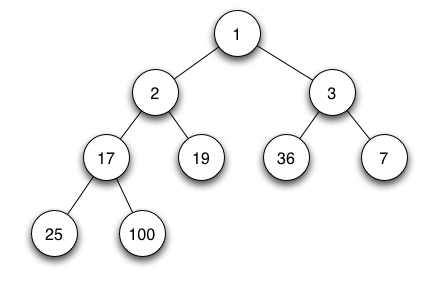
\includegraphics[width=0.6\textwidth]{min-heap.png}}
  \caption{Пример заполненной кучи для минимума}
  \label{pic:min-heap}
\end{figure} 
% \AgdaHide{
\begin{code}\>\<%
\\
\>\AgdaKeyword{module} \AgdaModule{HeapDef} \AgdaKeyword{where}\<%
\\
\>\AgdaKeyword{open} \AgdaKeyword{import} \AgdaModule{AgdaDescription}\<%
\\
\>\<\end{code}
}
\section{Тип данных для двоичной кучи}

\subsection{Заполнение дерева}
Куча заполняется элементами слева. Формализуем \cite{HeapFill} заполненность дерева:

\begin{definition}
Двоичное дерево высоты $h$ — \emph{полное} тогда и только тогда,
когда в нем $2^{h+1} - 1$ узлов.

Двоичное дерево высоты $h$ \emph{заполнено слева} тогда и только тогда,
когда выполняется ровно один из пунктов:
  \begin{itemize}
    \item дерево — пустое
    \item дерево — полное (то есть оба его поддерева — либо полные высоты $h-1$, либо пустые)
    \label{def:fill-nd}
    \item его левое поддерево — полное высотой $h-1$ и его правое поддерево — полное высотой $h-2$
    \item его левое поддерево — заполнено слева высотой $h-1$ и его правое поддерево — полное высотой $h-2$
    \item его левое поддерево — полное высотой $h-1$ и его правое поддерево — заполнено слева высотой $h-1$
  \end{itemize}
\end{definition}
Определим вспомогательный тип данных для обозначения заполненности дерева:
\begin{code}\>\<%
\\
\>\AgdaKeyword{data} \AgdaDatatype{TreeState} \AgdaSymbol{:} \AgdaPrimitiveType{Set} \AgdaKeyword{where}\<%
\\
\>[0]\AgdaIndent{2}{}\<[2]%
\>[2]\AgdaInductiveConstructor{full} \AgdaInductiveConstructor{almost} \AgdaSymbol{:} \AgdaDatatype{TreeState}\<%
\\
\>\<\end{code}
Теперь, используя этот тип данных как дополнительный индекс и
индексируя дерево его высотой, задать тип данных для заполненного слева дерева
\begin{code}\>\<%
\\
\>\AgdaKeyword{data} \AgdaDatatype{Tree} \AgdaSymbol{:} \AgdaSymbol{(}\AgdaBound{h} \AgdaSymbol{:} \AgdaDatatype{ℕ}\AgdaSymbol{)} \AgdaSymbol{→} \AgdaDatatype{TreeState} \AgdaSymbol{→} \AgdaPrimitiveType{Set} \AgdaKeyword{where}\<%
\\
\>[0]\AgdaIndent{2}{}\<[2]%
\>[2]\AgdaInductiveConstructor{et} \AgdaSymbol{:} \AgdaDatatype{Tree} \AgdaInductiveConstructor{zero} \AgdaInductiveConstructor{full} \AgdaComment{-- Пустое дерево}\<%
\\
\>[0]\AgdaIndent{2}{}\<[2]%
\>[2]\AgdaInductiveConstructor{nf} \AgdaSymbol{:} \AgdaSymbol{∀} \AgdaSymbol{\{}\AgdaBound{n}\AgdaSymbol{\}} \AgdaSymbol{→} \AgdaSymbol{(}\AgdaBound{a} \AgdaSymbol{:} \AgdaDatatype{Tree} \AgdaBound{n} \AgdaInductiveConstructor{full}\AgdaSymbol{)} \AgdaSymbol{→} \AgdaSymbol{(}\AgdaBound{b} \AgdaSymbol{:} \AgdaDatatype{Tree} \AgdaBound{n} \AgdaInductiveConstructor{full}\AgdaSymbol{)}\<%
\\
\>[2]\AgdaIndent{6}{}\<[6]%
\>[6]\AgdaSymbol{→} \AgdaDatatype{Tree} \AgdaSymbol{(}\AgdaInductiveConstructor{succ} \AgdaBound{n}\AgdaSymbol{)} \AgdaInductiveConstructor{full} \AgdaComment{-- Полное дерево}\<%
\\
\>[0]\AgdaIndent{2}{}\<[2]%
\>[2]\AgdaInductiveConstructor{nd} \AgdaSymbol{:} \AgdaSymbol{∀} \AgdaSymbol{\{}\AgdaBound{n}\AgdaSymbol{\}} \AgdaSymbol{→} \AgdaSymbol{(}\AgdaBound{a} \AgdaSymbol{:} \AgdaDatatype{Tree} \AgdaSymbol{(}\AgdaInductiveConstructor{succ} \AgdaBound{n}\AgdaSymbol{)} \AgdaInductiveConstructor{full}\AgdaSymbol{)} \AgdaSymbol{→} \AgdaSymbol{(}\AgdaBound{b} \AgdaSymbol{:} \AgdaDatatype{Tree} \AgdaBound{n} \AgdaInductiveConstructor{full}\AgdaSymbol{)}\<%
\\
\>[0]\AgdaIndent{6}{}\<[6]%
\>[6]\AgdaSymbol{→} \AgdaDatatype{Tree} \AgdaSymbol{(}\AgdaInductiveConstructor{succ} \AgdaSymbol{(}\AgdaInductiveConstructor{succ} \AgdaBound{n}\AgdaSymbol{))} \AgdaInductiveConstructor{almost} \AgdaComment{-- Полные поддеревья разной высоты}\<%
\\
\>[0]\AgdaIndent{2}{}\<[2]%
\>[2]\AgdaInductiveConstructor{nl} \AgdaSymbol{:} \AgdaSymbol{∀} \AgdaSymbol{\{}\AgdaBound{n}\AgdaSymbol{\}} \AgdaSymbol{→} \AgdaSymbol{(}\AgdaBound{a} \AgdaSymbol{:} \AgdaDatatype{Tree} \AgdaSymbol{(}\AgdaInductiveConstructor{succ} \AgdaBound{n}\AgdaSymbol{)} \AgdaInductiveConstructor{almost}\AgdaSymbol{)} \AgdaSymbol{→} \AgdaSymbol{(}\AgdaBound{b} \AgdaSymbol{:} \AgdaDatatype{Tree} \AgdaBound{n} \AgdaInductiveConstructor{full}\AgdaSymbol{)}\<%
\\
\>[0]\AgdaIndent{6}{}\<[6]%
\>[6]\AgdaSymbol{→} \AgdaDatatype{Tree} \AgdaSymbol{(}\AgdaInductiveConstructor{succ} \AgdaSymbol{(}\AgdaInductiveConstructor{succ} \AgdaBound{n}\AgdaSymbol{))} \AgdaInductiveConstructor{almost} \AgdaComment{-- Правое поддерево — полное}\<%
\\
\>[0]\AgdaIndent{2}{}\<[2]%
\>[2]\AgdaInductiveConstructor{nr} \AgdaSymbol{:} \AgdaSymbol{∀} \AgdaSymbol{\{}\AgdaBound{n}\AgdaSymbol{\}} \AgdaSymbol{→} \AgdaSymbol{(}\AgdaBound{a} \AgdaSymbol{:} \AgdaDatatype{Tree} \AgdaBound{n} \AgdaInductiveConstructor{full}\AgdaSymbol{)} \AgdaSymbol{→} \AgdaSymbol{(}\AgdaBound{b} \AgdaSymbol{:} \AgdaDatatype{Tree} \AgdaBound{n} \AgdaInductiveConstructor{almost}\AgdaSymbol{)}\<%
\\
\>[0]\AgdaIndent{6}{}\<[6]%
\>[6]\AgdaSymbol{→} \AgdaDatatype{Tree} \AgdaSymbol{(}\AgdaInductiveConstructor{succ} \AgdaBound{n}\AgdaSymbol{)} \AgdaInductiveConstructor{almost} \AgdaComment{-- Левое поддерево — полное}\<%
\\
\>\<\end{code}
Для удобства будем называть заполненное слева дерево, индексированное \DC{almost}
\emph{неполным}.

\section{Вставка элементов}
\label{sec:insert}

\subsection{Вставка элементов в полное дерево}
\label{sec:finsert}
\subsection{Вставка элементов в неполное дерево}
\label{sec:ainsert}

\section{Удаление элементов}
\label{sec:delete}
\subsection{Удаление из полного дерева}
\subsection{Удаление из неполного дерева}

\input{latex/HeapTries.tex}

\section{Выводы по главе \ref{chapter2}}
Разработаны типы данных для представления структуры данных двоичная куча.

% \chapter{Результаты} 
\label{chapter3}

В данном разделе описываются результаты экспериментов, демонстрирующих работу предложенного метода генерации покрывающего набора тестов. 

\section{Покрытие тестами модельных задач}
Исследования проводились на пяти модельных задачах, взятых с сайта инструментального средства Microsoft Pex \texttt{http://pexforfun.com}. 

\subsection{Описание модельных задач}
Для каждой задачи приводится исходный код на языке \textit{C\#}, описывается способ кодирования теста и оператор мутации. Для построения покрывающего набора 
тестов использовалась \texttt{(1+1)}-эволюционная стратегия.

В рассматриваемых задачах при применении оператора мутации для изменения целого числа \texttt{x} к нему добавлялось число вида $(r(19) - 9) \cdot 10 ^{r(10)}$, 
где $r(a)$~--- случайное целое число в диапазоне $[0, a)$. Если \texttt{x} должен находиться в диапазоне от $-10^5$ до $10^5$, то он заменяется на $\max(-10^5, 
\min(10^5, x + (r(19) - 9) \cdot 10^{r(4)}))$. 

\subsubsection{Задача 1}
\label{pex01}
Код тестируемой программы приведен на листинге~\ref{lst:pex-1-source}. Наиболее сложным для покрытия является случай, когда сумма элементов массива равняется 
42. В качестве тестов генерируются целочисленные массивы длины шесть. Оператор мутации выбирает случайный элемент массива и изменяет его описанным ранее 
способом.

\begin{snippet}[language=C++,caption={Код задачи 1 с сайта pexforfun},label={lst:pex-1-source}]
using System;

public class Program {
  //#What values of v to cause the exception? Ask Pex to find out!#
  public static int Puzzle(int[] v) {
    int sum = 0;
    foreach (int x in v)
      sum += x;
    if (sum == 42)
      throw new Exception("hidden bug!");
    return sum;
  }
}
\end{snippet}

\subsubsection{Задача 2}

Код тестируемой программы приведен на листинге~\ref{lst:pex-2-source}. Сложность данной задачи заключается в покрытии случая, когда элемент списка, следующий 
за указанным, на единицу больше. Тестом является список, состоящий из шести целых чисел, и число из множества $\{0, 1, 2, 3, 4\}$~--- в качестве индекса 
элемента в списке. Оператор мутации случайным образом выбирает другой индекс, либо изменяет элемент списка, выбранный случайным образом.  

\begin{snippet}[language=C++,caption={Код задачи 2 с сайта pexforfun},label={lst:pex-2-source}]
using System;
using System.Collections.Generic;

public class Program
{
  //# What values of list and i can cause exceptions? Ask Pex to find out!#
  public static void Puzzle(List<int> list, int i)
  {
    if (list[i] + 1 == list[i + 1])
      throw new Exception("hidden bug!"); 
  }
}
\end{snippet}

\subsubsection{Задача 3}
                   
Код тестируемой программы приведен на листинге~\ref{lst:pex-3-source}. Сложнее всего покрыть случай, когда сумма выбранного элемента массива и 27277 равняется 
42. Тест представляется в виде массива из шести целых чисел и числа из множества $\{0, 1, 2, 3, 4, 5\}$~--- индекса элемента в массиве. Оператор мутации 
случайным образом выбирает другой индекс, либо изменяет элемент массива, выбранный случайным образом.  

\begin{snippet}[language=C++,caption={Код задачи 3 с сайта pexforfun},label={lst:pex-3-source}]
using System;

public class Program {
  //# What values of v and i can cause an exception? Ask Pex to find out!#
  public static void Puzzle(int[] v, int i) {
    if (v[i] + 27277 == 42)
      throw new Exception("hidden bug!"); 
  }
}
\end{snippet}

\subsubsection{Задача 4}
                   
Код тестируемой программы приведен на листинге~\ref{lst:pex-4-source}. Чтобы полностью покрыть данную задачу, необходимо подобрать корень линейного уравнения. 
В качестве теста берется целое число в диапазоне от $-10^5$ до $10^5$. Оператор мутации изменяет текущее решение описанным ранее образом.

\begin{snippet}[language=C++,caption={Код задачи 4 с сайта pexforfun},label={lst:pex-4-source}]
using System;

public class Program 
{
  public static void Puzzle(int x)
  {
    // What value of x solves this equation? Ask Pex to find out!
    if (x * 3 + 27 == 153)
      Console.WriteLine("equation solved");
  }
}
\end{snippet}

\subsubsection{Задача 5}
                                                            
Код тестируемой программы приведен на листинге~\ref{lst:pex-5-source}. Сложнее всего покрыть тестом строку, в которой производится вывод на консоль.
Это эквивалентно решению нелинейного уравнения второй степени в целых числах с двумя переменными и наличием ограничений. Тест представляется в виде кортежа из 
двух целых чисел в диапазоне от $-10^5$ до $10^5$. Оператор мутации изменяет одно из них.

\begin{snippet}[language=C++,caption={Код задачи 5 с сайта pexforfun},label={lst:pex-5-source}]
using System;

public class Program {
  public static void Puzzle(int x, int y) {
    //# What values of x and y solve this equation? Ask Pex to find out!#
    if (x >= 0 && x <= 100 &&
        y >= 0 && y <= 100 &&
        x * y - 37 * y + 71 * x - 2627 == 0)        
      Console.WriteLine("equation solved"); 
  }
}
\end{snippet}

\subsection{Результаты эксперимента}

Для каждой из рассмотренных задач было проведено 1000 запусков эволюционного алгоритма. В результате каждого из запусков был сгенерирован покрывающий набор 
тестов. В таблице~\ref{pexres} приведены минимальное, среднее и максимальное число вычислений функции приспособленности (ФП).

\begin{table}[h!]
\caption{Число вычислений ФП на модельных задачах} \label{pexres}
\begin{tabular}{|p{5em}|c|c|c|}
\hline
№ задачи & ФП, мин. & ФП, среднее & ФП, макс. \\\hline
%Pex #01
1  & 33  &  340 & 1449 \\\hline
%Pex #02
2 & 2  &  660& 3909 \\\hline
%Pex #03
3  & 286  &  2604 & 13078 \\\hline
%Pex #04
4  & 20  &  201 & 679 \\\hline
%Pex #05
5  & 298  &  1429 & 4086 \\\hline
\end{tabular}
\end{table}

Покрытие модельных задач было осуществлено с помощью тестов, сгенерированных случайным образом. При этом, чтобы было возможным полное покрытие заданного кода, 
пространство поиска тестов было уменьшено. Так, например, для задачи \ref{pex01} массив заполнялся целыми числами в диапазоне от $-5 \cdot 10^5$ до $5 \cdot 
10^5$. При этом на каждом запуске генерировалось в $10$ раз больше тестов, чем максимальное число вызовов ФП для соответствующей задачи. В таблице 
\ref{randompex} приведены полученные результаты, усредненные по 1000 запускам.

\begin{table}
\caption{Результаты покрытия модельных задач случайными тестами} \label{randompex}
\begin{tabular}{|p{5em}|c|c|}
\hline
№ задачи & Покрытие, \% & Число тестов на каждом запуске\\\hline
% Pex #01
1 & 75.3 & 15000\\\hline
% Pex #02
2 & 52.7 & 40000\\\hline
% Pex #03
3 & 55.6 & 130000\\\hline
% Pex #04
4 & 51.4 & 7000\\\hline
% Pex #05
5 & 66.7 & 41000\\\hline
\end{tabular}
\end{table}

Из результатов эксперимента можно сделать вывод, что применение эволюционного алгоритма для генерации тестов, покрывающих заданные строки кода, весьма 
эффективно даже для сложных условий.

\section{Покрытие тестами олимпиадных задач}
Исследования проводились на основе задачи  Huzita Axiom 6, предложенной на NEERC 2011. 

\subsection{Условие задачи}
Заданы две прямые $l_1$ и $l_2$ и две точки $p_1$ и $p_2$. Необходимо найти прямую, по которой можно сложить плоскость так, что точка $p_1$ попадет на прямую 
$l_1$, а точка $p_2$ попадет на прямую $l_2$. Прямые задаются с помощью двух точек. Пример условия задачи приведен на рис.~\ref{huzita_pic}.
\begin{figure}[h!]
 \center{\includegraphics[width=0.8\textwidth]{huzita.pdf}}
 \caption{Иллюстрация к задаче  Huzita Axiom 6}
 \label{huzita_pic}
\end{figure}

\subsection{Описание эксперимента}

Для тестирования решений задачи был разработан интерфейс \textit{Solution}, приведенный на листинге~\ref{lst:huzita_solution}. Решения реализуют данный 
интерфейс. Входные данные(тест) передаются в виде строки, а результат выдается в виде списка строк.

\begin{snippet}[language=Java,caption={Интерфейс решения задачи Huzita Axiom 6},label={lst:huzita_solution}]
public interface Solution {
    public List<String> solve(String input) throws IOException;
}
\end{snippet}

Для построения покрывающего набора тестов использовалась \texttt{(1+1)}-эволюционная стратегия. Пример конфигурации ЭА, приведен на 
листинге~\ref{lst:huzita_config}.

\begin{snippet}[language=Scala,caption={Конфигурация эволюционного алгоритма для задачи  Huzita Axiom 6},label={lst:huzita_config}]
class HuzitaConfig[C <: Solution](val cl : Class[C], override val maxGenerationCount : Long) 
  extends  TargetAwareComputationStateImpl
  with CoverageConfig[TestData, DistDiffFitness]
  with OnePlusOneES
  with TraceProvider
  with Mutation
  with FastRandomDelegate
  with CoverageFitnessComparator.LeastDistLeastAbsDiff[DistDiffFitness]
  with GenotypeGenerator
  with GenotypeWrapper
  with TotalFitnessCallCount
{
  private[this] def nestedClasses(top : Class[_]) : Seq[Class[_]] = {
    top.getDeclaredClasses.toSeq.map(x => nestedClasses(x)).flatten :+ top
  }

  override def targetMethods: Seq[Method] = nestedClasses(cl).map(_.getDeclaredMethods).flatten

  override def targetConstructors: Seq[Constructor[_]] = nestedClasses(cl).map(_.getDeclaredConstructors).flatten

  def newGenotype(): TestData = TestData.genTestData()

  private[this] lazy val mh =  MethodHandles.lookup().findVirtual(cl, "solve", MethodType.methodType(classOf[java.util.List[String]], classOf[String]))

  def wrap(genotype: TestData): Seq[AnyRef] = genotype.toTestString :: Nil

  def mutate(source: TestData): TestData = source.mutate()

  def evaluateFitness(genotype: TestData): DistDiffFitness = computeFitness(wrap(genotype))

  protected def invoke(args: Seq[AnyRef]) {
    mh.invokeWithArguments(cl.newInstance() +: args : _*)
  } 
} 
\end{snippet}

Точка задается двумя целочисленными координатами. При мутации точки изменяются обе ее координаты. Линия определяется с помощью двух точек, и при мутации 
изменяется каждая из них. Тест, используемый в качестве особи ЭА, задается с помощью двух прямых~--- $l_1$ и $l_2$~--- и двух точек~---$p_1$ и $p_2$. 
Рассматривается пять типов операторов мутации тестовых данных.
Мутируют:
\begin{enumerate}
 \item либо $l_1$ и $p_1$, либо $l_2$ и $p_2$;
 \item либо $l_1$ и $l_2$, либо $p_1$ и $p_2$;
 \item одна из $l_1$, $l_2$, $p_1$, $p_2$;
 \item все прямые и все точки;
 \item одна из $l_1$ и $p_1$ и одна из $l_2$ и $p_2$.
\end{enumerate}

\subsection{Результаты}

Для каждого эксперимента было проведено по 1000 запусков. В таблицах~\ref{huzita_10_res}, \ref{huzita_100_res} и \ref{huzita_1000_res} приведены результаты 
работы ЭА, когда координаты точек лежат в диапазоне от $-10$ до 10, от $-100$ до 100 и от $-1000$ до 1000 соответственно. В первой колонке указан номер 
оператора мутации, во второй~--- среднее число вычислений ФП, а в третьей~--- усредненный процент покрытия кода. Можно видеть, что лучшие результаты были 
получены при использовании пятого оператора мутации.

\begin{table}[h!]
\caption{ЭА, диапазон от $-10$ до 10} \label{huzita_10_res}
\begin{tabular}{|p{5em}|c|c|}
\hline
№ мутации &  ФП, среднее & Покрытие, \% \\\hline
1  & $2,5 \cdot 10^4$ &  95,8 \\\hline
2  & $2,9 \cdot 10^4$  &  95  \\\hline
3  & $4,5 \cdot 10^4$  &  89,3 \\\hline
4  & $2,5 \cdot 10^4$  &  95,9 \\\hline
5  & $2,2 \cdot 10^4$  &   \cellcolor{purpur}96,6 \\\hline
\end{tabular}
\end{table}

\begin{table}[h!]
\caption{ЭА, диапазон от $-100$ до 100} \label{huzita_100_res}
\begin{tabular}{|p{5em}|c|c|}
\hline
№ мутации &  ФП, среднее & Покрытие, \% \\\hline
1  & $5,7 \cdot 10^5$ & 87,3 \\\hline
2  & $4,7 \cdot 10^5$  &  89,7  \\\hline
3  & $5,7 \cdot 10^5$  &  87,3 \\\hline
4  & $6,7 \cdot 10^5$  &  88,3 \\\hline
5  & $4,2 \cdot 10^5$  &  \cellcolor{purpur}91,3 \\\hline
\end{tabular}
\end{table}

\begin{table}[h!]
\caption{ЭА, диапазон от $-1000$ до 1000} \label{huzita_1000_res}
\begin{tabular}{|p{5em}|c|c|}
\hline
№ мутации &  ФП, среднее & Покрытие, \% \\\hline
1  & $7,4 \cdot 10^5$  & 81,7 \\\hline
2  & $6,7 \cdot 10^5$  &  87,3  \\\hline
3  & $6,2 \cdot 10^5$ & 88 \\\hline
4  & $7,9 \cdot 10^5$  &  79,3 \\\hline
5  & $5,9 \cdot 10^5$ &  \cellcolor{purpur}90 \\\hline
\end{tabular}
\end{table}

В таблице~\ref{huzita_random_res} приведены результаты покрытия кода случайными тестами в сравнении с результатами ЭА. В первой колонке указан диапазон 
координат, во второй~--- число случайно генерируемых тестов, в третьей~--- усредненный процент покрытия кода случайными тестами, а в четвертой~--- лучший 
усредненный процент покрытия кода с помощью ЭА.

\begin{table}
\caption{Покрытие решения Huzita Axiom 6 случайными тестами} \label{huzita_random_res}
\begin{tabular}{|p{7em}|c|c|c|}
\hline
Диапазон &  Число тестов & Покрытие, \% & Покрытие ЭА, \%\\\hline
$-10$ до 10  & $5 \cdot 10^5$  & \cellcolor{purpur}97,7  & 96,6 \\\hline
$-100$ до 100 & $10^6$  &  80,3 & \cellcolor{purpur}91,3 \\\hline
$-1000$ до 1000  & $10^6$  & 74,3 & \cellcolor{purpur}90 \\\hline
\end{tabular}
\end{table}

Из результатов эксперимента можно сделать вывод, что время и качество работы ЭА сильно зависит от выбора оператора мутации. При увеличении множества допустимых 
тестов, ЭА работает стабильнее и достигает лучших результатов, чем случайная генерация тестов.

\section{Выводы по главе \ref{chapter3}}
Были проведены эксперименты, демонстрирующие работу предложенного подхода для автоматизированного покрытия кода тестами на основе эволюционных алгоритмов. В 
результате экспериментов, проведенных на модельных задачах, было получено, что разработанный метод эффективен для покрытия даже сложных условий. Также 
применимость разработанного подхода была протестирована на олимпиадной задаче Huzita~Axiom~6. Было получено, что эффективность данного метода сильно зависит от 
выбора эволюционных операторов. Можно видеть, что при увеличении множества допустимых тестов результаты предложенного подхода превосходят результаты, 
полученные при покрытии кода случайными тестами.

% \startconclusionpage

Представленный в данной работе подход к представлению инвариантов —
по одному конструктору на каждый случай инварианта —
приводит к неприятному разрастанию функций по обработке структуры данных.
Но данный подход позволил написать простые доказательства
с помощью интерактивного редактора, использующего систему типов
для указания типа требуемого терма.
Хотелось бы уметь обобщать такие представления инвариантов для
упрощения доказательств и уменьшения объема кода.


\printbibliography

% \startappendices
% \chapter{Обзор предметной области}
\label{chapter1}

В программировании структуры данных позволяют упростить хранение и обработку
множество однотипных и/или логически связанных данных.
Задача структур данных — облегчить написание программ для программистов и
ускорить обработку данных.

\section{Структуры данных}
Структуры данных используются в программировании для абстрагирования
обработки связанных и однородных данных.

Часто используемые структуры данных включаются в стандартные библиотеки
языков программирования.

\subsection{Функциональные структуры данных}

Главное отличие функциональных структур данных от императивных \cite{OkasakiBook}
заключается в неиспользовании разрушающих обновлений (то есть присваиваний).
При обновлении структуры данных все измененные части создаются заново.

\section{Индуктивные семейства и зависимые типы}

\begin{definition}
\emph{Индуктивное семейство} \cite{DybjerIndFam}— это семейство типов данных,
которые могут зависеть от других типов и значений.

Тип или значение, от которого зависит зависимый тип, называют \emph{индексом}.
\end{definition}

Одной из областей применения индуктивных семейств являются системы интерактивного
доказательства теорем.

Индуктивные семейства позволяют формализовать математические структуры,
кодируя утверждения о структурах в них самих, тем самым перенося сложность из
доказательств в определения.

% \section{Существующие подходы}
В работах \cite{OkasakiThesis, McBridePivotal} приведены различные подходы
к построению функциональных структур данных.

Пример задания инвариантов для
структуры данных — тип данных для хранения баланса в AVL-дереве \cite{AVLTree}.
\newline
\AgdaHide{
\begin{code}\>\<%
\\
\>\AgdaKeyword{module} \AgdaModule{AVLBalance} \AgdaKeyword{where}\<%
\\
\>[0]\AgdaIndent{2}{}\<[2]%
\>[2]\AgdaKeyword{open} \AgdaKeyword{import} \AgdaModule{AgdaDescription}\<%
\\
\>[0]\AgdaIndent{2}{}\<[2]%
\>[2]\AgdaKeyword{infix} \AgdaNumber{4} \_∼\_\<%
\\
\>[0]\AgdaIndent{2}{}\<[2]%
\>[2]\AgdaFunction{testˡ} \AgdaSymbol{:} \AgdaDatatype{ℕ}\<%
\\
\>[0]\AgdaIndent{2}{}\<[2]%
\>[2]\AgdaFunction{testˡ} \AgdaSymbol{=} \AgdaInductiveConstructor{succ} \AgdaInductiveConstructor{zero}\<%
\\
\>\<\end{code}
}
Если $m \sim n$, то разница между $m$ и $n$ не больше чем один:
\begin{code}\>\<%
\\
\>[0]\AgdaIndent{2}{}\<[2]%
\>[2]\AgdaKeyword{data} \AgdaDatatype{\_∼\_} \AgdaSymbol{:} \AgdaDatatype{ℕ} \AgdaSymbol{→} \AgdaDatatype{ℕ} \AgdaSymbol{→} \AgdaPrimitiveType{Set} \AgdaKeyword{where}\<%
\\
\>[2]\AgdaIndent{4}{}\<[4]%
\>[4]\AgdaInductiveConstructor{∼+} \AgdaSymbol{:} \AgdaSymbol{∀} \AgdaSymbol{\{}\AgdaBound{n}\AgdaSymbol{\}} \AgdaSymbol{→} \<[21]%
\>[21]\AgdaBound{n} \AgdaDatatype{∼} \AgdaNumber{1} \AgdaFunction{+} \AgdaBound{n}\<%
\\
\>[2]\AgdaIndent{4}{}\<[4]%
\>[4]\AgdaInductiveConstructor{∼0} \AgdaSymbol{:} \AgdaSymbol{∀} \AgdaSymbol{\{}\AgdaBound{n}\AgdaSymbol{\}} \AgdaSymbol{→} \<[21]%
\>[21]\AgdaBound{n} \AgdaDatatype{∼} \AgdaBound{n}\<%
\\
\>[2]\AgdaIndent{4}{}\<[4]%
\>[4]\AgdaInductiveConstructor{∼-} \AgdaSymbol{:} \AgdaSymbol{∀} \AgdaSymbol{\{}\AgdaBound{n}\AgdaSymbol{\}} \AgdaSymbol{→} \AgdaNumber{1} \AgdaFunction{+} \AgdaBound{n} \AgdaDatatype{∼} \AgdaBound{n}\<%
\\
\>\<\end{code}


\section{Agda}
\textit{Agda}~\cite{AgdaLang}~---  чистый функциональный язык программирования с зависимыми типами.
В Agda есть поддержка модулей:
\begin{code}\>\<%
\\
\>\AgdaKeyword{module} \AgdaModule{AgdaDescription} \AgdaKeyword{where}\<%
\\
\>\<\end{code} В коде на Agda широко используются символы Unicode.
Тип натуральных чисел — \D{ℕ}.
\begin{code}\>\<%
\\
\>\AgdaKeyword{data} \AgdaDatatype{ℕ} \AgdaSymbol{:} \AgdaPrimitiveType{Set} \AgdaKeyword{where}\<%
\\
\>[0]\AgdaIndent{2}{}\<[2]%
\>[2]\AgdaInductiveConstructor{zero} \AgdaSymbol{:} \AgdaDatatype{ℕ}\<%
\\
\>[0]\AgdaIndent{2}{}\<[2]%
\>[2]\AgdaInductiveConstructor{succ} \AgdaSymbol{:} \AgdaDatatype{ℕ} \AgdaSymbol{→} \AgdaDatatype{ℕ}\<%
\\
\>\<\end{code} \AgdaHide{
\begin{code}\>\<%
\\
\>\AgdaSymbol{\{-\#} \AgdaKeyword{BUILTIN} NATURAL \AgdaDatatype{ℕ} \AgdaSymbol{\#-\}}\<%
\\
\>\AgdaSymbol{\{-\#} \AgdaKeyword{BUILTIN} ZERO \AgdaInductiveConstructor{zero} \AgdaSymbol{\#-\}}\<%
\\
\>\AgdaSymbol{\{-\#} \AgdaKeyword{BUILTIN} SUC \AgdaInductiveConstructor{succ} \AgdaSymbol{\#-\}}\<%
\\
\>\<\end{code}
}
В Agda функции можно определять как mixfix операторы.
Пример — сложение натуральных чисел:
\begin{code}\>\<%
\\
\>\AgdaFunction{\_+\_} \AgdaSymbol{:} \AgdaDatatype{ℕ} \AgdaSymbol{→} \AgdaDatatype{ℕ} \AgdaSymbol{→} \AgdaDatatype{ℕ}\<%
\\
\>\AgdaInductiveConstructor{zero} \AgdaFunction{+} \AgdaBound{b} \AgdaSymbol{=} \AgdaBound{b}\<%
\\
\>\AgdaInductiveConstructor{succ} \AgdaBound{a} \AgdaFunction{+} \AgdaBound{b} \AgdaSymbol{=} \AgdaInductiveConstructor{succ} \AgdaSymbol{(}\AgdaBound{a} \AgdaFunction{+} \AgdaBound{b}\AgdaSymbol{)}\<%
\\
\>\<\end{code}
Символы подчеркивания обозначают места для аргументов.
% Система типов \textit{Agda} позволяет ... 
% В отличие от \textit{Haskell}, в \textit{Agda} имеется ... 

Зависимые типы позволяют определять типы, зависящие (индексированные) от значений
других типов. Пример — список, индексированный своей длиной:
\begin{code}\>\<%
\\
\>\AgdaKeyword{data} \AgdaDatatype{Vec} \AgdaSymbol{(}\AgdaBound{A} \AgdaSymbol{:} \AgdaPrimitiveType{Set}\AgdaSymbol{)} \AgdaSymbol{:} \AgdaDatatype{ℕ} \AgdaSymbol{→} \AgdaPrimitiveType{Set} \AgdaKeyword{where}\<%
\\
\>[0]\AgdaIndent{2}{}\<[2]%
\>[2]\AgdaInductiveConstructor{nil} \<[7]%
\>[7]\AgdaSymbol{:} \AgdaDatatype{Vec} \AgdaBound{A} \AgdaInductiveConstructor{zero}\<%
\\
\>[0]\AgdaIndent{2}{}\<[2]%
\>[2]\AgdaInductiveConstructor{cons} \AgdaSymbol{:} \AgdaSymbol{∀} \AgdaSymbol{\{}\AgdaBound{n}\AgdaSymbol{\}} \AgdaSymbol{→} \AgdaBound{A} \AgdaSymbol{→} \AgdaDatatype{Vec} \AgdaBound{A} \AgdaBound{n} \AgdaSymbol{→} \AgdaDatatype{Vec} \AgdaBound{A} \AgdaSymbol{(}\AgdaInductiveConstructor{succ} \AgdaBound{n}\AgdaSymbol{)}\<%
\\
\>\<\end{code}
В фигурные скобки заключаются неявные аргументы.

Такое определение позволяет нам описать функцию $ \F{head} $ для такого списка, которая не может бросить исключение:
\begin{code}\>\<%
\\
\>\AgdaFunction{head} \AgdaSymbol{:} \AgdaSymbol{∀} \AgdaSymbol{\{}\AgdaBound{A}\AgdaSymbol{\}} \AgdaSymbol{\{}\AgdaBound{n}\AgdaSymbol{\}} \AgdaSymbol{→} \AgdaDatatype{Vec} \AgdaBound{A} \AgdaSymbol{(}\AgdaInductiveConstructor{succ} \AgdaBound{n}\AgdaSymbol{)} \AgdaSymbol{→} \AgdaBound{A}\<%
\\
\>\<\end{code}
У аргумента функции $ \F{head} $ тип $ \D{Vec}\,A\,(\DC{succ}\,n) $, то есть вектор, в котором есть хотя бы один элемент.
Это позволяет произвести сопоставление с образцом только по конструктору $ \DC{cons} $:
\begin{code}\>\<%
\\
\>\AgdaFunction{head} \AgdaSymbol{(}\AgdaInductiveConstructor{cons} \AgdaBound{a} \AgdaBound{as}\AgdaSymbol{)} \AgdaSymbol{=} \AgdaBound{a}\<%
\\
\>\<\end{code}



\section{Выводы по главе \ref{chapter1}}
Рассмотрены некоторые существующие подходы к построению структур данных
с использованием индуктивных семейств.
Кратко описаны особенности языка программирования \textit{Agda}.

% \begin{appendices}
%     \chapter{Some Appendix}
%     The contents...
% \end{appendices}

\end{document}
